\chapter{MOEA Operator Convergence}
\label{appendix-operatorconvergence}

In addition to overall epsilon progress and hypervolume convergence, the likelihood of each operator being selected for a generation was tracked throughout the search process. The likelihood of selection is updated after each generation based on how successful that operator was at identifying non-dominated policy alternatives. To contrast with the five operators available to the auto-adaptive $\epsilon$-NSGAII algorithm, traditional $\epsilon$-NSGAII uses a single operator: simulated binary crossover (SBX) variator + polynomial mutation (PM) mutator \citep{Reed2013}.

\section{Intertemporal}
Each of the analyses using the intertemporal model, shown in \cref{fig:operatorconvergence-inter} quickly converge to using a uniform mutation (UM) almost 100 percent of the time. This indicates that the best operator for convergence with respect to the intertemporal problem is not the SBX operator used by traditional $\epsilon$-NSGAII, but another operator entirely. This result matches the failure of several MOEAs, including $\epsilon$-NSGAII, to find a strong set of policy alternatives \citep{Ward2015}. This same study also found Borg to be the only successful MOEA of the ones tested with respect to the intertemporal problem variation. Given the search success found in this study, the proposed auto-adaptive $\epsilon$-NSGAII algorithm remains a promising alternative to Borg. The SBX and parent-centric crossover (PCX) operators maintain some likelihood of use for a subset of the search repetitions. However, the maximum likelihood for both after the initial startup does not reach higher than the original likelihood of use of 15 percent, so use of those operators continued to be uncommon. 

\section{Planned adaptive DPS}
The planned adaptive DPS operator selection, shown in \cref{fig:operatorconvergence-planned} did not converge to a single operator like the intertemporal analyses did. The most commonly used operators in each of the intertemporal analyses are the PCX, SBX, and UM. There is wide variation between each repetition of the search process as to which operator is more likely to be selected, however.

\section{Direct Policy Search}
The DPS-based analyses and corresponding operator selection convergences are shown in \cref{fig:operatorconvergence-dps}. The multi-scenario MORDM and MORO analyses display similar behavior as with the planned adaptive DPS model variation. There is some interesting behavior in the MORDM analysis, however. As \cref{fig:convergences-dps} showed, the epsilon progress trend reaches a steady level initially and then begins to increase again at around 50,000 function executions, leveling out as progress reaches 100,000 function executions. Correspondingly with that behavior are the likelihood trends of both the UM and SBX operators. Initially, The UM operator is significantly more likely to be selected than the SBX operator. Then, at around 50,000 function executions, there is a transition between the two operators, and the SBX operator becomes more likely to be selected than the UM operator. This information indicates that the auto-adaptive $\epsilon$-NSGAII algorithm realized that it was no longer able to make progress with the UM operator, but that the SBX operator was still discovering new non-dominated policy alternatives, and was able to transition between the two operators to continue progressing in the search. However, referring to the hypervolume convergence in \cref{fig:convergences-dps}, the epsilon-based progress made using the SBX operator did not result in alternatives that contributed to an increase in hypervolume of the non-dominated set. 

\begin{figure}[ht]
    \centering
    \captionsetup{width=0.85\textwidth}
    
    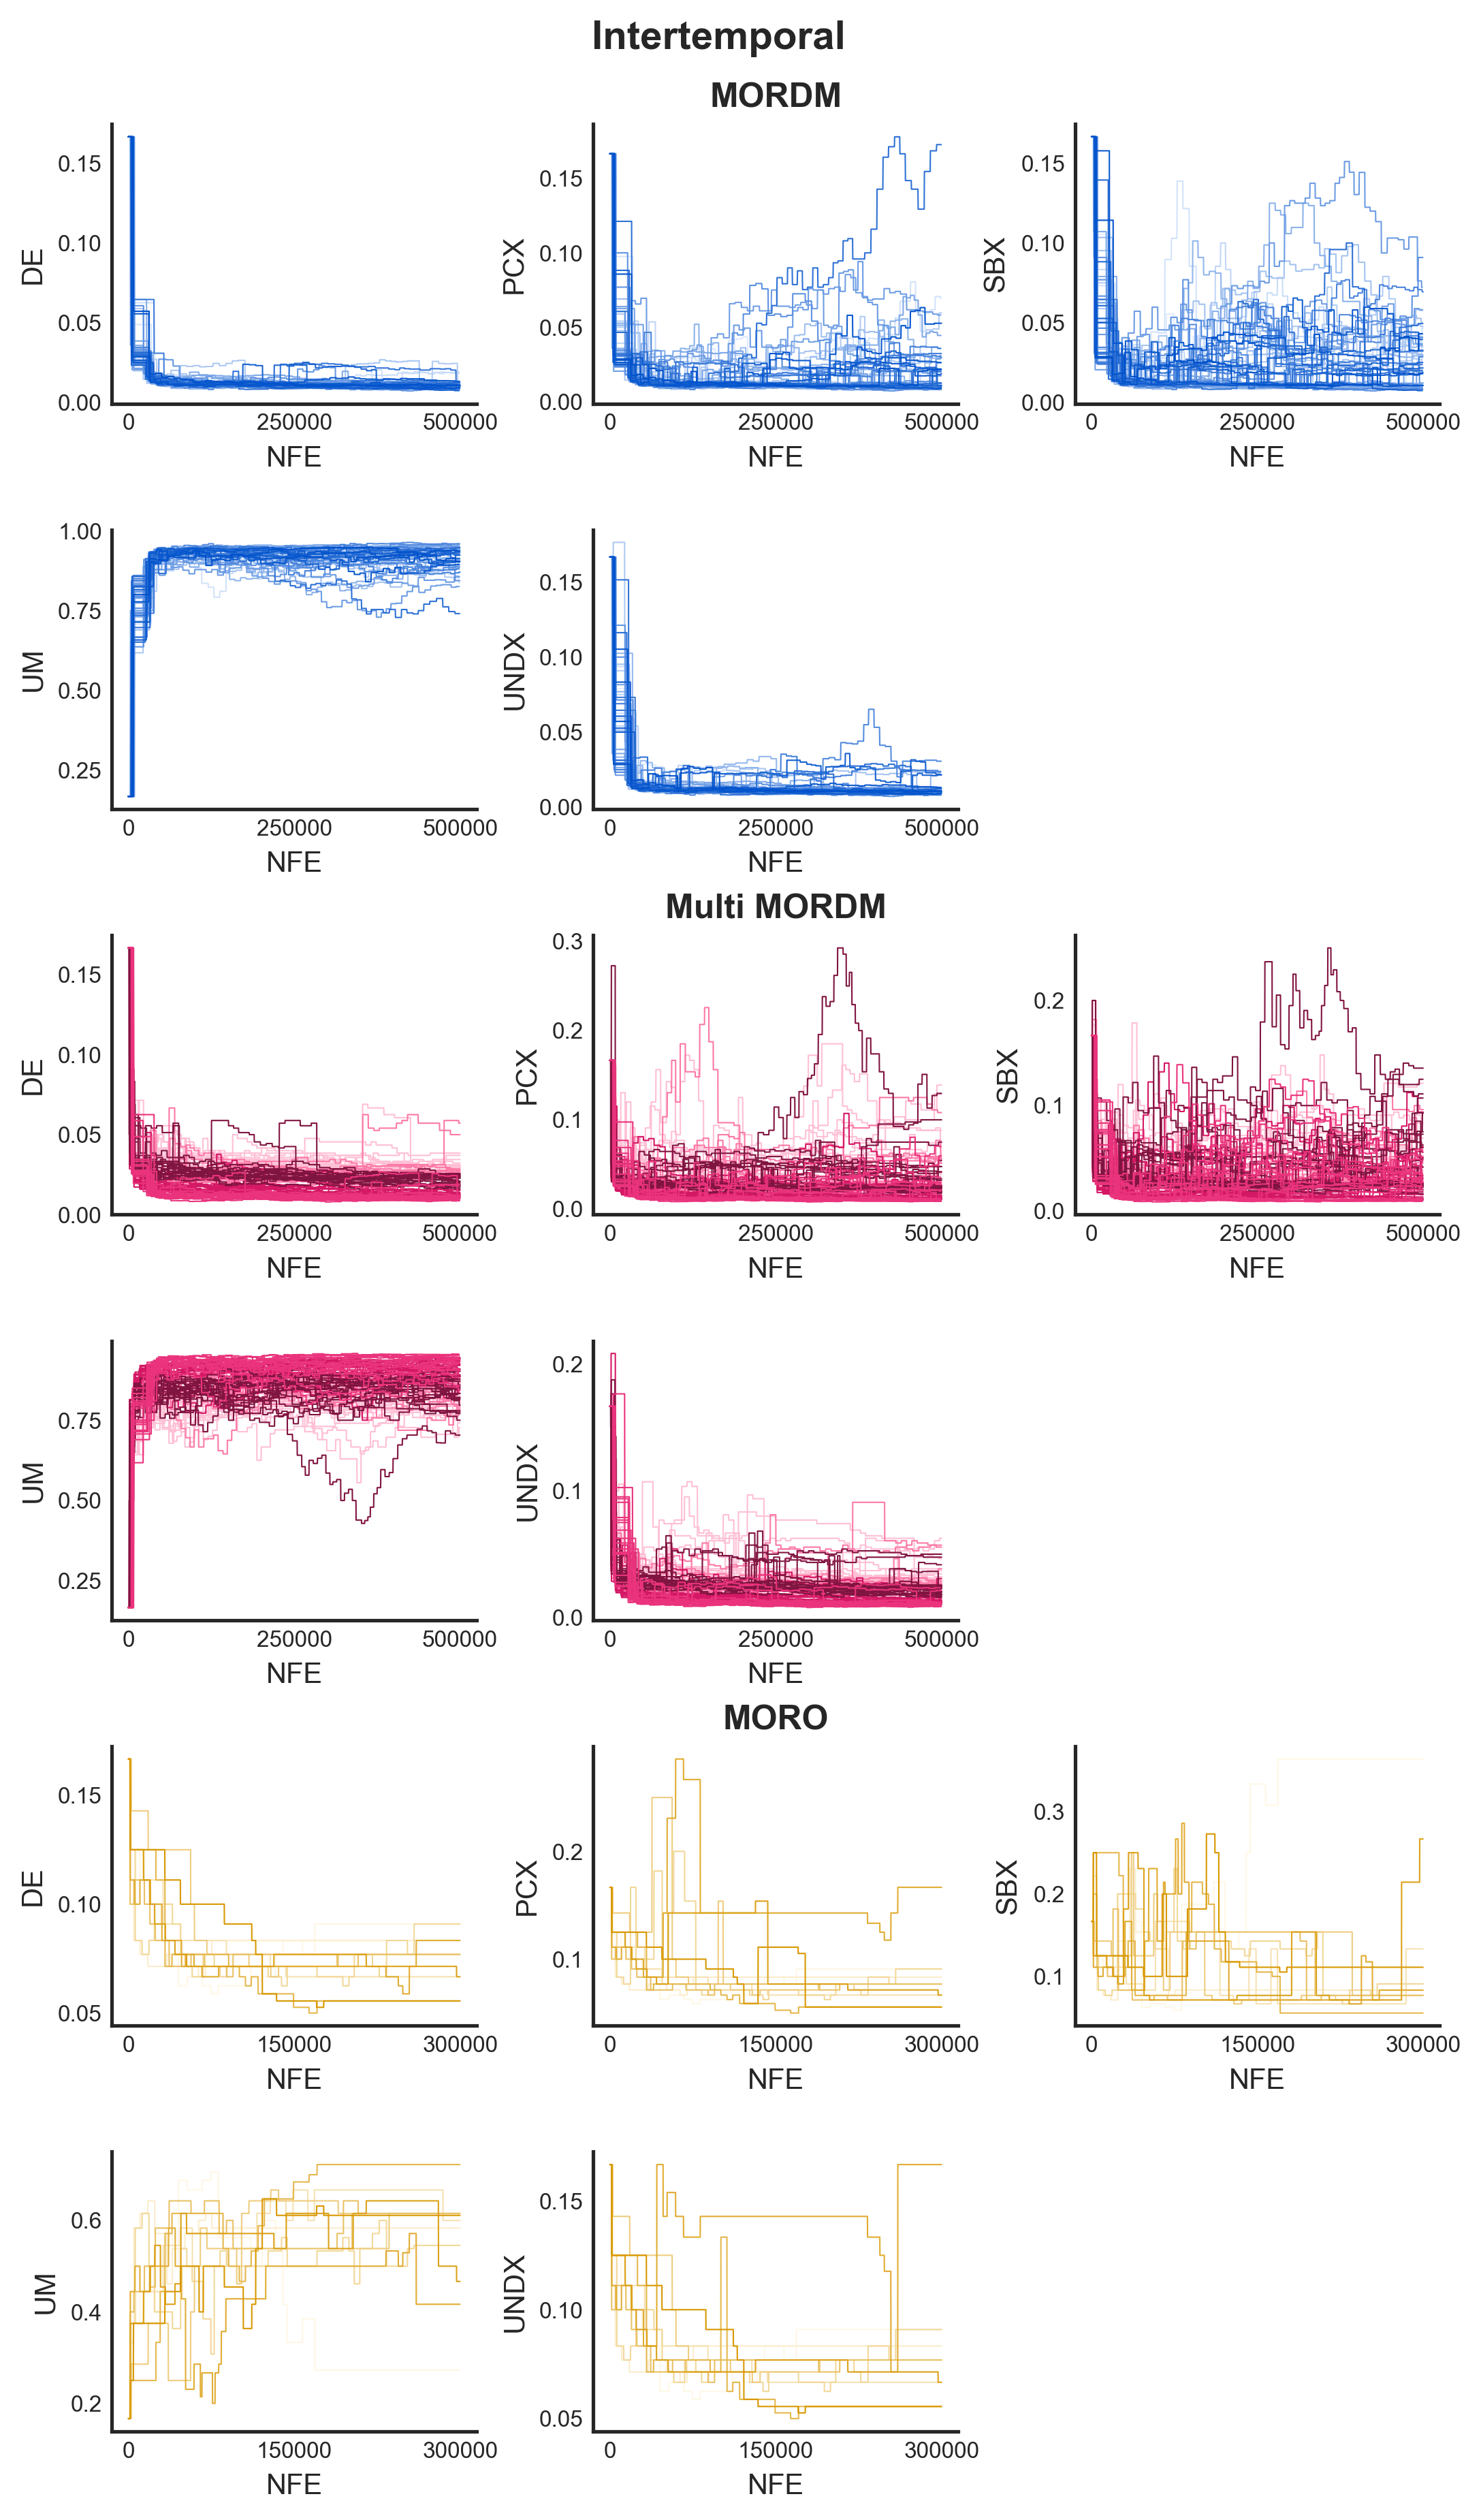
\includegraphics[width=0.85\textwidth]{appendices/operator_convergence/operatorconvergence_inter}
    \caption[Operator convergence for the intertemporal model variation]{The convergence of the five operators used in the Auto-Adaptive $\epsilon$-NSGAII operator selection for all methods using the intertemporal lake model variation.}
    \label{fig:operatorconvergence-inter}
\end{figure}

\begin{figure}[ht]
    \centering
    \captionsetup{width=0.85\textwidth}
    
    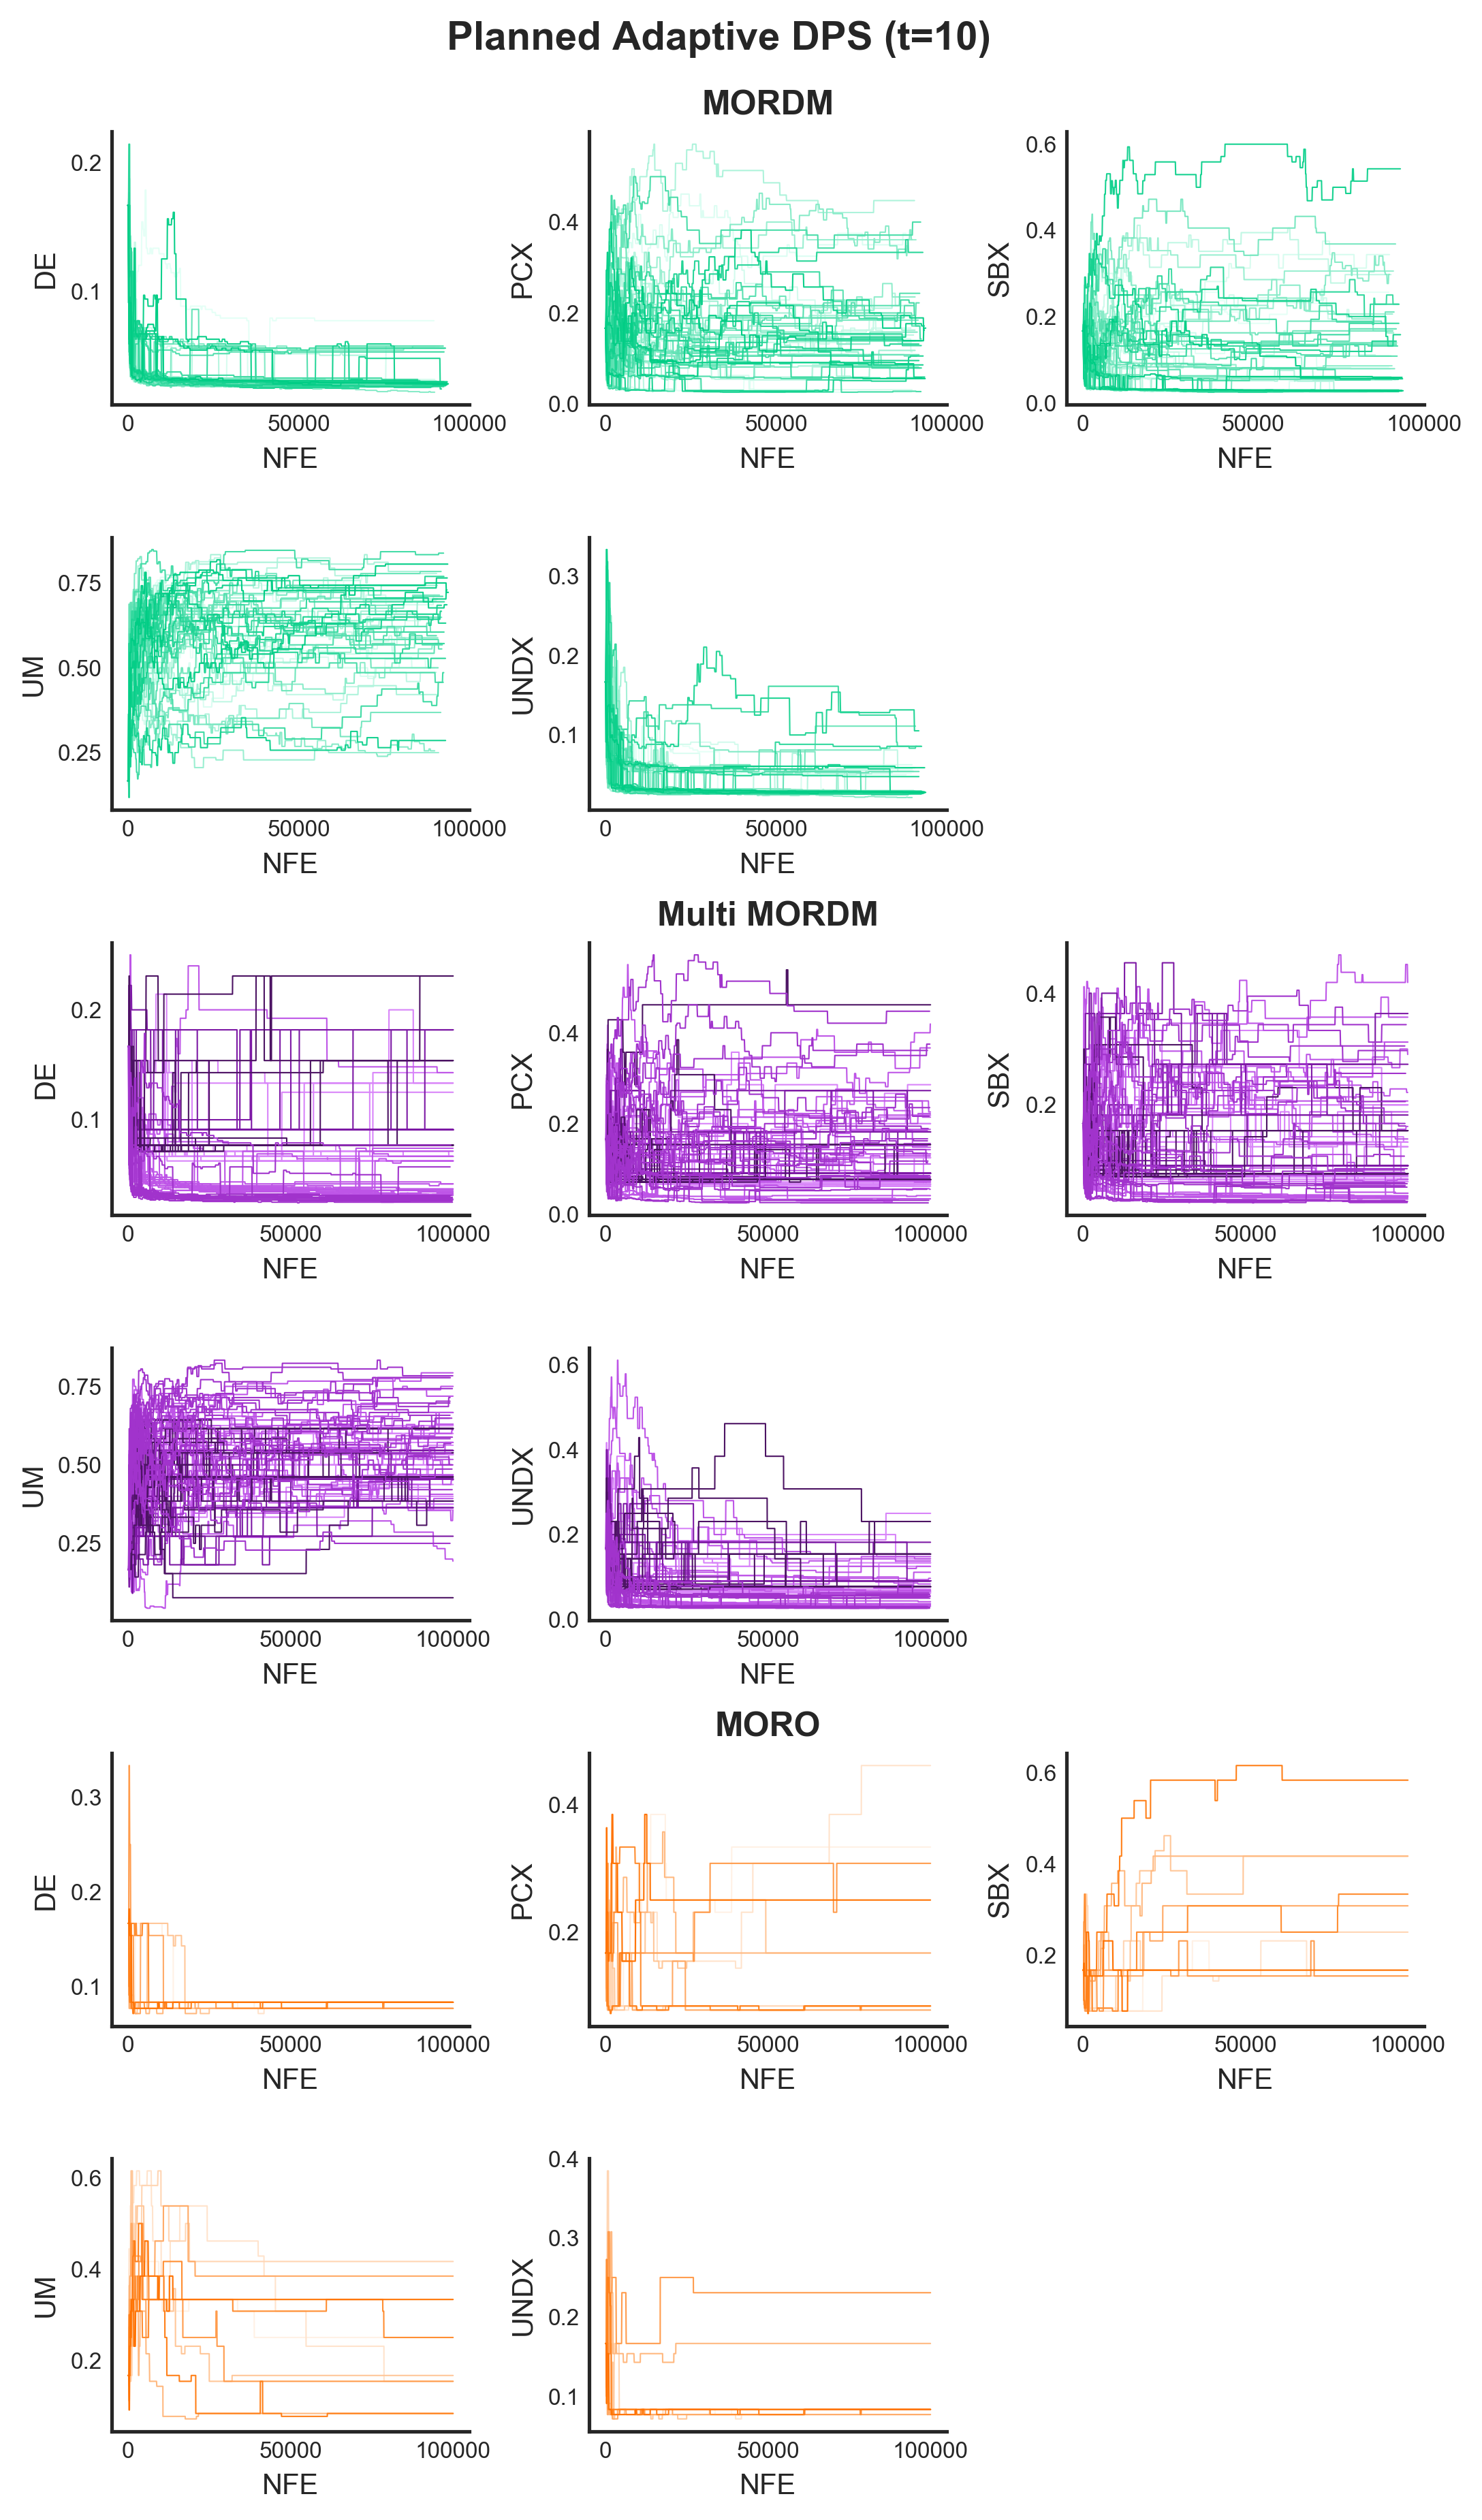
\includegraphics[width=0.85\textwidth]{appendices/operator_convergence/operatorconvergence_planned}
    \caption[Operator convergence for the planned adaptive DPS model variation]{The convergence of the five operators used in the Auto-Adaptive $\epsilon$-NSGAII operator selection for all methods using the planned adaptive DPS lake model variation.}
    \label{fig:operatorconvergence-planned}
\end{figure}

\begin{figure}[ht]
    \centering
    \captionsetup{width=0.85\textwidth}
    
    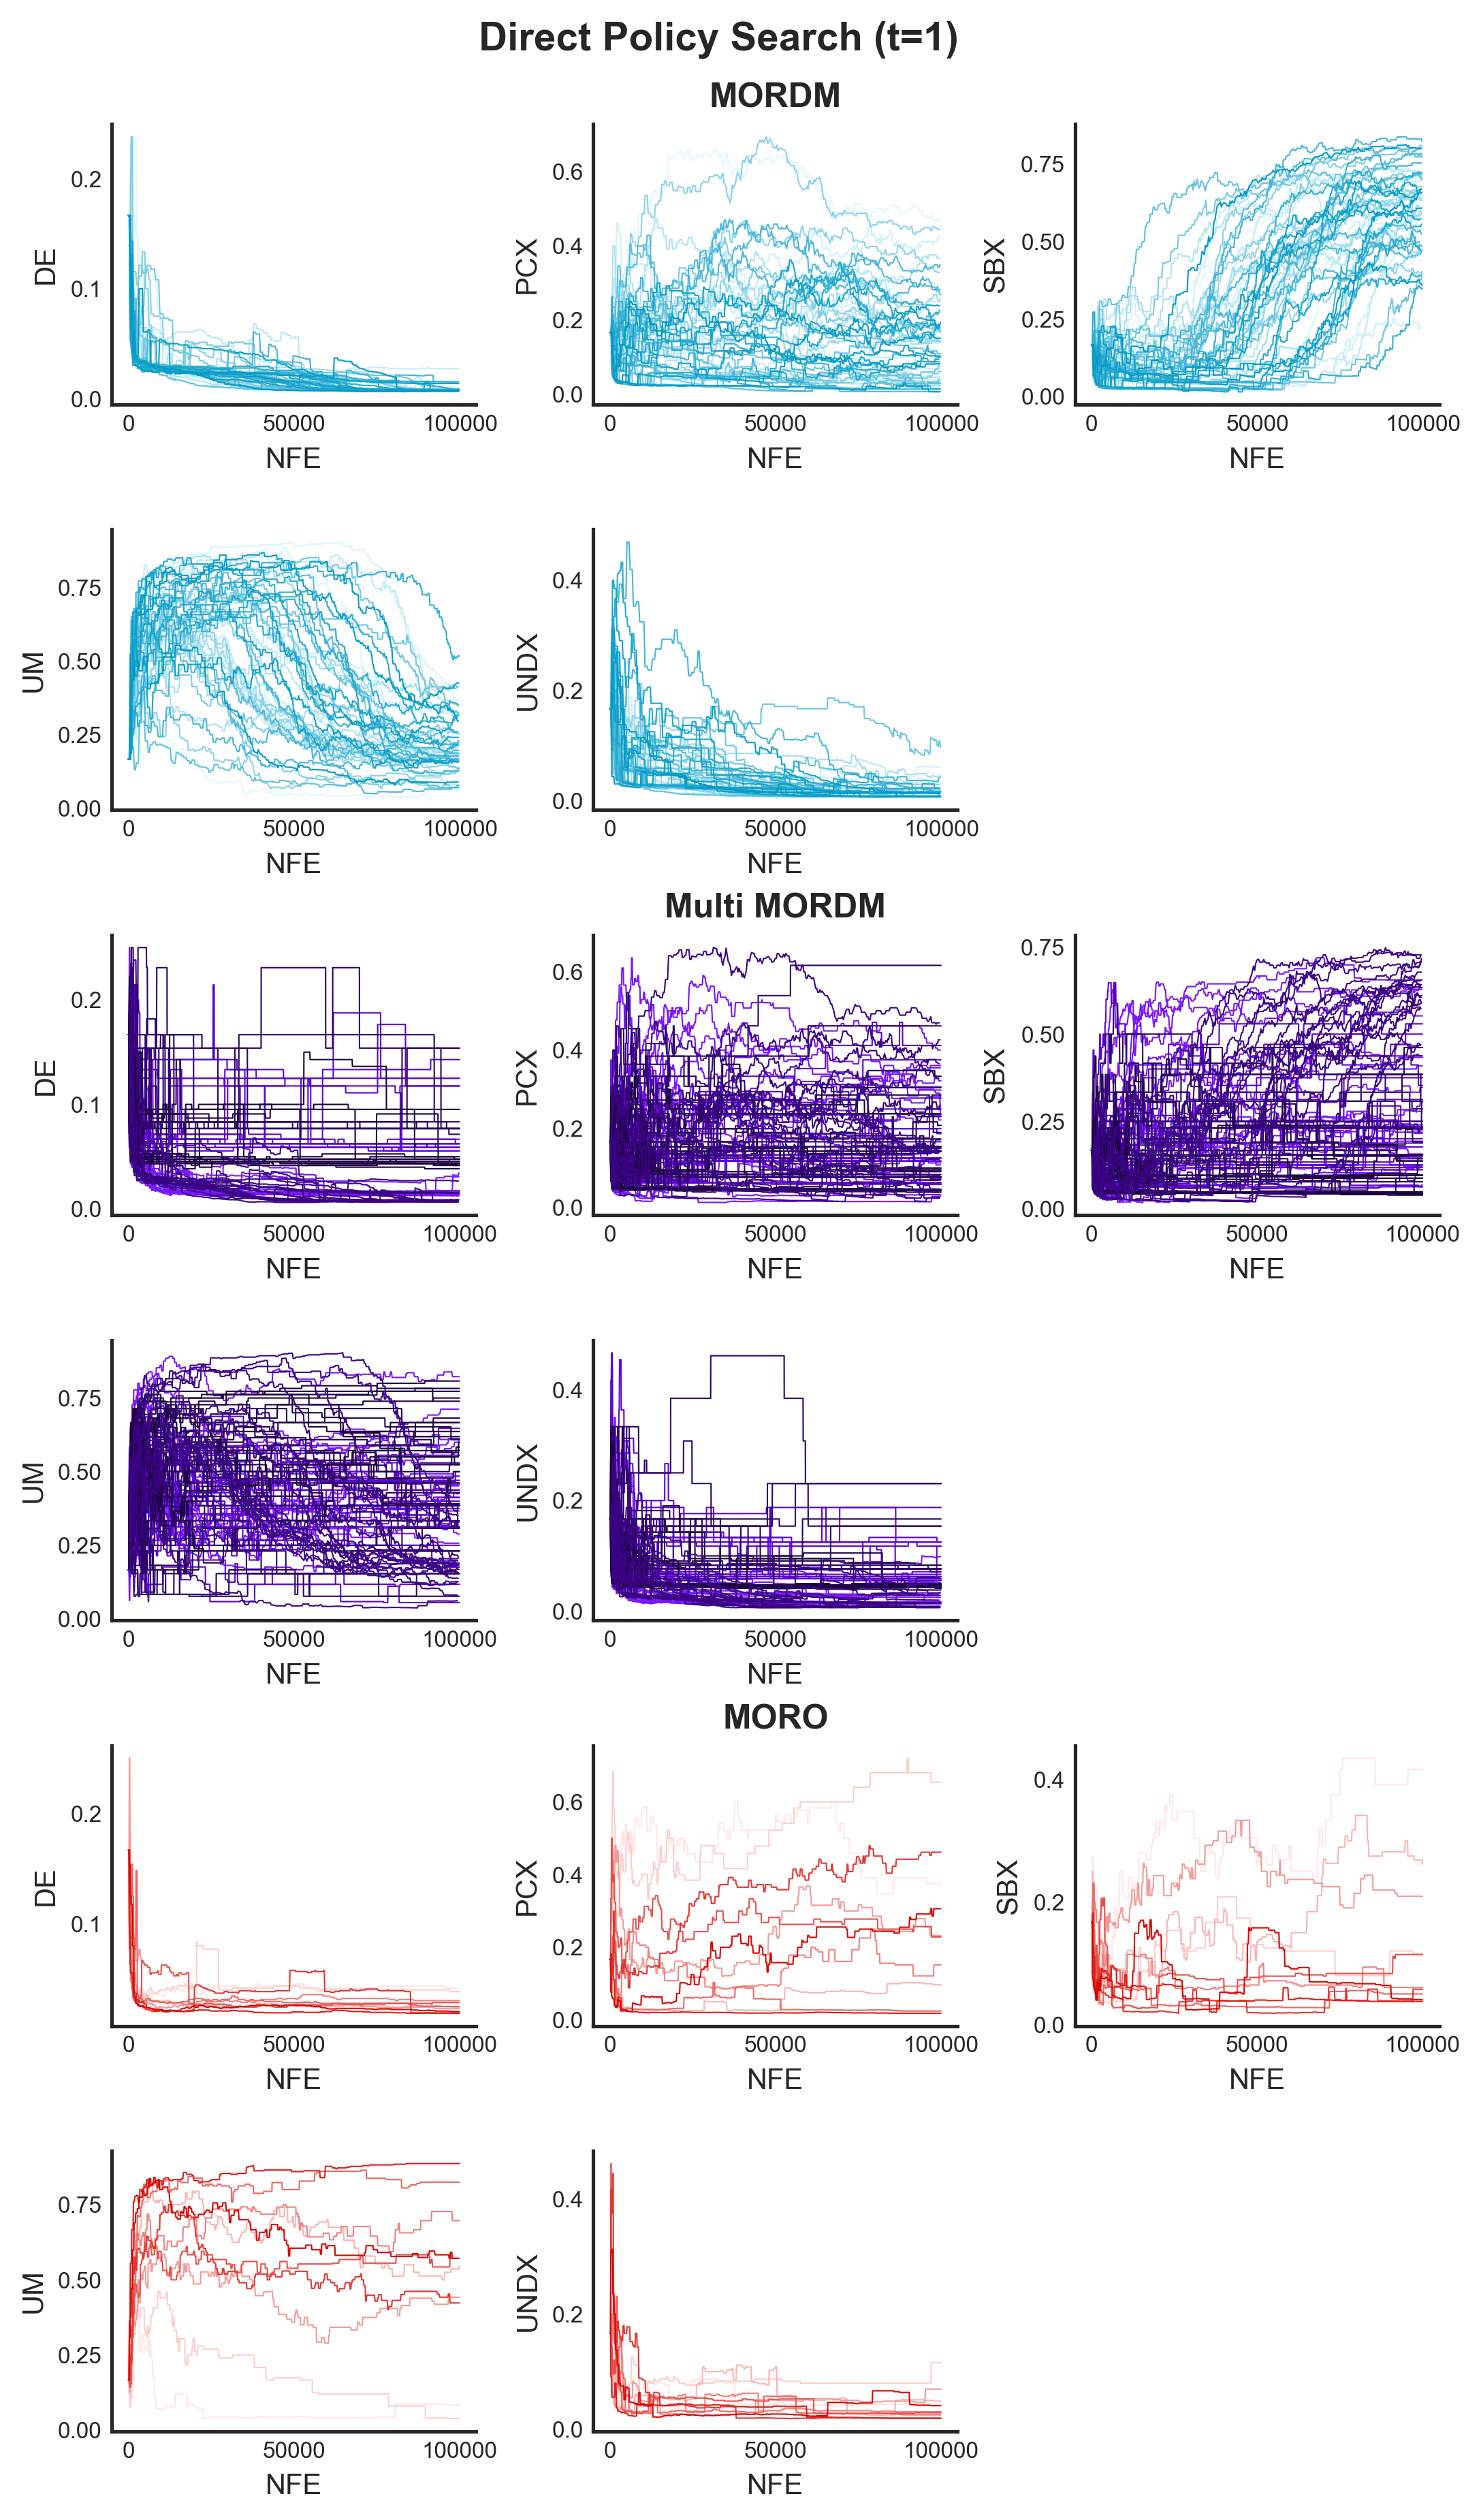
\includegraphics[width=0.85\textwidth]{appendices/operator_convergence/operatorconvergence_dps}
    \caption[Operator convergence for the DPS model variation]{The convergence of the five operators used in the Auto-Adaptive $\epsilon$-NSGAII operator selection for all methods using the DPS lake model variation.}
    \label{fig:operatorconvergence-dps}
\end{figure}